\section{引言}
\label{sec:intro}

煤炭是我国最主要的一次能源，近年煤炭产量有所缩减，但 2000 年产量仍保持在 10 亿吨。由于煤炭在我国化石能源资源总量中占 95\%，石油和天然气的储采比低，分别为 21 和 40，因此估计到二十一世纪中叶，煤炭在一次能源结构中所占的比例仍难低于 50\%。所以煤的地球化学性质，特别是煤中有害元素及有害有机化合物及其对大气、土壤和水域的环境危害，对人体健康的影响，日益受到重视$^{[1-3,5]}$。煤中伴生元素环境地球化学的研究可为我国煤炭资源、环境与可持续发展的决策提供一定的科学依据。

\subsection{煤中有害元素对环境和人体健康的危害}

煤中有害元素引起的生物中毒和环境污染在许多用煤国家都已发生。如美国大气硒污染主要来源是燃煤，燃煤引起的大气硒排放量占总量的 62\%。燃煤过程向大气的排汞量占了人为总量的大部分，成为大气中汞的最大污染源。大气汞通过干湿沉降返回到表生生态环境中，加速了汞在水生生态系统食物链中富集强度和速度，对人类的生存构成了潜在威胁。在北欧 and 北美，酸雨沉降区的一些偏远湖泊中，一些鱼体中汞含量高的惊人，远远超过了世界卫生组织建议的地区食用水产品的汞含量标准。美国近 10 年来集中研究了燃煤造成的汞污染。煤烟是大气中砷的主要来源，著名的伦敦上空的烟雾，其大气中的砷含量为 0.04 $\sim$ 0.14$\mu$g/m3。原捷克斯洛伐克燃煤电厂排放的 Pb、As 已造成附近儿童骨骼生长延缓。美国近年正研究燃煤造成的 As 污染，并拟降低大气及水域中可造成 As 污染的下限值。

\begin{figure}[H]
    \centering
    
\includegraphics[width=0.8\textwidth]{../figure/图片1.png}
    \caption{煤中化学元素从环境到有机体作用路线示意图}
    \label{fig:pathway}
    \centerline{Fig.\ 1.1 Sketch map of ways of chemical elements on organism}
\end{figure}

\subsection{煤中伴生元素的有关术语和分类}

\subsubsection{元素的含量分类}

在常见的地球化学文献中，人们常将 O、Si、Al、Fe、Ca、Mg、Na、K 和 Ti 等 9 种元素（它们的地壳丰度共占 99\%左右）称之为常量元素或主要元素，而把这 9 种元素以外的元素统称为微量元素或痕量元素、杂质元素、副元素、稀有元素、次要元素等（Trace, Minor, Micro, Rare, Oligo Elements），它们在岩石中含量一般在 1\%或 0.1\%以下。

目前还没有建立微量元素地球化学分类的统一标准，分类方案也因研究对象和目的不同而异。目前普遍采用程介克（1986）的分类方案（表 1.1）$^{[3]}$。

\begin{table}[H]
    \centering
    \caption{元素含量的术语及其含量界限(程介克，1986)}
    \zihao{5}
    \centerline{Table 1.1 Terms of elements and their content limits (Cheng Kejie, 1986)}
    \begin{tabular}{cccL{7.5cm}}
        \toprule
        \multicolumn{2}{c}{含量} & \multirow{2}{*}{有关术语} \\
        (\%) & ($\mu$g/g) & \\
        \midrule
        1 ~ 100 & $10^4 \sim 10^6$ & 常量元素 (Major Element 或 Macroelement) \\
        0.01 ~ 1 & 100 ~ 10000 & 微量元素 (Minor Element 或 Microelement) \\
        0.0001 ~ 0.01 & 1 ~ 100 & 痕量元素 (Trace Element) \\
        < 0.0001 & < 1 & 超痕量元素 (Ultratrace Element) \\
        \bottomrule
    \end{tabular}
\end{table}

然而，常量元素和微量元素的区分是相对的，常因研究的对象和目的而异。煤是物质成分极其复杂的固体可燃有机岩，用现有的分析技术手段可以从煤中检测到 66 种元素，从煤样品、燃煤产物和煤层气样品中检测到 86 种元素（地壳中可供统计的元素共 88 种），只有 Ac 和 Pa 这 2 种短寿命的放射性元素在煤、煤燃烧产物和煤层气中未曾检测到。在所检测到的元素中，作者把 H、C、N、O、Na、Mg、Al、Si、S、K、Ca 和 Fe 等 12 种元素称之为常量元素（major elements），它们在煤中的含量一般超过 0.1\%；其它元素在大多数煤中的含量低于 0.1\%，称之为微量元素（minor elements）（图 1.2）。是间接检测，尚未有一种行之有效的直接检测方法，更谈不上某元素在各种赋存状态中各占的百分比例。二是研究煤炭在开采、运输、堆放、洗选加工、燃烧等过程中有害元素侵入环境的机制和规律，正如前所述，煤是一种特殊的岩石，在其加工利用过程中，可以使得本来一些并不富集的元素得以富集后对环境或人类健康造成危害，特别是燃煤过程中有害元素在飞灰中的迁移和富集尤其引人注意。三是研究和开发脱除或降低煤中伴生有害元素的技术，从而达到控制和预防煤中伴生元素对环境和人类身体健康的危害，主要涉及到煤洁净利用技术的工艺方面。

发展趋势：一是开始研究全球煤中有害元素分布规律，如捷克著名学者 Bouška 等（1999）总结了全球 31 个国家褐煤中硫及微量元素含量的分布，主要有害元素的样品都在千个以上（其中我国仅 10 个左右）$^{[51]}$；美国著名的专家 Finkelman 正在力争建立全球煤中毒害元素的地球化学数据库；二是研究煤中有害物质对人类健康的影响，美国 Orem 等（1999）对巴尔干半岛上褐煤淋出的有害有机化合物对地方性肾脏病的影响等$^{[89]}$；2001 年在捷克召开的第 9 届煤田地质会议上，就有一些煤中有害元素与病理学关系方面的新研究成果，引起了与会学者极大兴趣$^{[90]}$。三是一些学者开始注重低温热液流体作用下煤中伴生元素的地球化学行为，把流体动力学的原理应用于煤中物质，特别是毒害元素的迁移、转化和富集规律的研究。把流体动力学的原理应用于煤中物质，特别是毒害元素的迁移、转化和富集规律的研究。注重流/岩反应、流/流反应以及沉积有机物自身的有机反应、有机物-水-岩石多相反应和有细菌参与的生物有机化学反应。流体是物质迁移和转化的主要载体，任德贻等（1999）剖析了几种煤中伴生有害元素的富集成因特点$^{[88]}$，无不与流体有关。把流体动力学的原理应用于煤中物质，特别是毒害元素的迁移、转化和富集规律的研究。把流体动力学的原理应用于煤中物质，特别是毒害元素的迁移、转化和富集规律的研究。近年来低温地球化学的快速发展为此项研究提供了新的思路和可靠的理论参考。

总结国内外研究现状和发展趋势，作者认为煤中伴生元素地球化学的研究在以下几个方面需进一步加强：

(1) 我国学者比较系统、深入的研究煤中毒害元素局限于华北的东部和中部、贵州省、四川省及东北个别煤田，积累了不少煤中有害元素分布的基础数据，掌握了一些有害元素的局部的富集规律，但与先进国家相比，全国积累的系统研究数据较少，并且多数集中于煤中伴生元素高异常区，往往使人产生误解，认为中国煤中有害元素普遍偏高。把流体动力学的原理应用于煤中物质，特别是毒害元素的迁移、转化和富集规律的研究。把流体动力学的原理应用于煤中物质，特别是毒害元素的迁移、转化和富集规律的研究。因此，全面评价我国煤炭资源及其环境效应，充分合理地利用丰富的煤炭资源，已有的研究成果和数据仍显不足。

(2) 对煤中有害微量元素在有机质聚积、成岩、各种变质作用、热液作用过程中的富集机理及其地质背景探讨尚显不足。对源岩、围岩、岩浆热液活动产物的地球化学研究有待深入。我国黔西、滇东、湘南等地岩浆、构造热液作用是导致局部地区煤中有害元素富集的主要因素。把流体动力学的原理应用于煤中物质，特别是毒害元素的迁移、转化和富集规律的研究。华北地区区域岩浆热变质作用是决定煤级分布的主因，但其对煤中有害元素富集的影响研究甚少。所以从含煤盆地（煤产地）所处的区域地质、地球化学背景和地质发展史角度进行理论总结，归纳出煤中有害元素富集的成因类型或地质模式，尚须深入研讨。

\begin{table}[H]
    \centering
    \caption{1989-2005 年统计表}
    \label{tab:stats}
    \zihao{5}
    \centerline{Table 1.2 The data in coal mine from 1989 to 2005}
    \begin{tabular*}{\textwidth}{@{\extracolsep{\fill}}ccccccc}
        \toprule
        \multirow{2}{*}{年份} & \multicolumn{2}{c}{合计} & \multicolumn{2}{c}{1 以上} & \multicolumn{2}{c}{其中：3 以上} \\
        \cmidrule(lr){2-3} \cmidrule(lr){4-5} \cmidrule(lr){6-7}
        & 数 1 & 数 2 & 数 3 & 数 4 & 数 5 & 数 6 \\
        \midrule
        1989 &      & 7625 & 40 & 631  & 2  & 87  \\
        1990 &      & 7360 & 51 & 941  & 5  & 227 \\
        1991 &      & 6412 & 36 & 751  & 5  & 308 \\
        1992 &      & 5992 & 42 & 821  & 6  & 244 \\
        1993 & 3859 & 6244 & 50 & 989  & 8  & 383 \\
        1994 & 4021 & 7239 & 70 & 1297 & 9  & 448 \\
        1995 & 3619 & 6907 & 59 & 1042 & 6  & 289 \\
        1996 & 2655 & 6556 & 73 & 1378 & 8  & 419 \\
        1997 & 3288 & 7083 & 95 & 1930 & 16 & 761 \\
        1998 & 2867 & 6302 & 79 & 1541 & 10 & 495 \\
        1999 & 3216 & 6469 & 75 & 1235 & 8  & 316 \\
        2000 & 2720 & 5796 & 75 & 1405 & 6  & 370 \\
        2001 & 3082 & 5670 & 49 & 1015 & 8  & 373 \\
        2002 & 4344 & 6995 & 56 & 1167 & 9  & 417 \\
        2003 & 4088 & 6702 & 51 & 1061 & 7  & 360 \\
        \bottomrule
    \end{tabular*}
\end{table}

\begin{center}
    \zihao{5}
    \makebox[0.85\textwidth]{\dotfill} \\
    \makebox[0.85\textwidth]{\dotfill} \\
    \makebox[0.85\textwidth]{\dotfill} \\
    \makebox[0.85\textwidth]{\dotfill} \\
    \makebox[0.85\textwidth]{\dotfill} \\
    \makebox[0.85\textwidth]{\dotfill} \\
    \makebox[0.85\textwidth]{\dotfill} \\
    \makebox[0.85\textwidth]{\dotfill} \\
    \makebox[0.85\textwidth]{\dotfill} \\
    \makebox[0.85\textwidth]{\dotfill}
\end{center}

\begin{flushright}
    \zihao{-5} 续表 1.2
\end{flushright}
\vspace{-1.5em}
\begin{table}[H]
    \centering
    \zihao{5}
    \begin{tabular*}{\textwidth}{@{\extracolsep{\fill}}ccccccc}
        \toprule
        \multirow{2}{*}{年份} & \multicolumn{2}{c}{合计} & \multicolumn{2}{c}{1 以上} & \multicolumn{2}{c}{其中：3 以上} \\
        \cmidrule(lr){2-3} \cmidrule(lr){4-5} \cmidrule(lr){6-7}
        & 数 1 & 数 2 & 数 3 & 数 4 & 数 5 & 数 6 \\
        \midrule
             & 3641 & 6027 & 42 & 1008 & 7  & 487 \\
             & 3306 & 5938 & 58 & 1739 & 11 & 961 \\
        \bottomrule
    \end{tabular*}
    \vspace{0.1cm}
    \raggedleft\zihao{-5}（备注：本表数据来自国家有关统计资料）
\end{table}

\clearpage
\subsubsection{技术路线}

\begin{figure}[H]
    \centering
    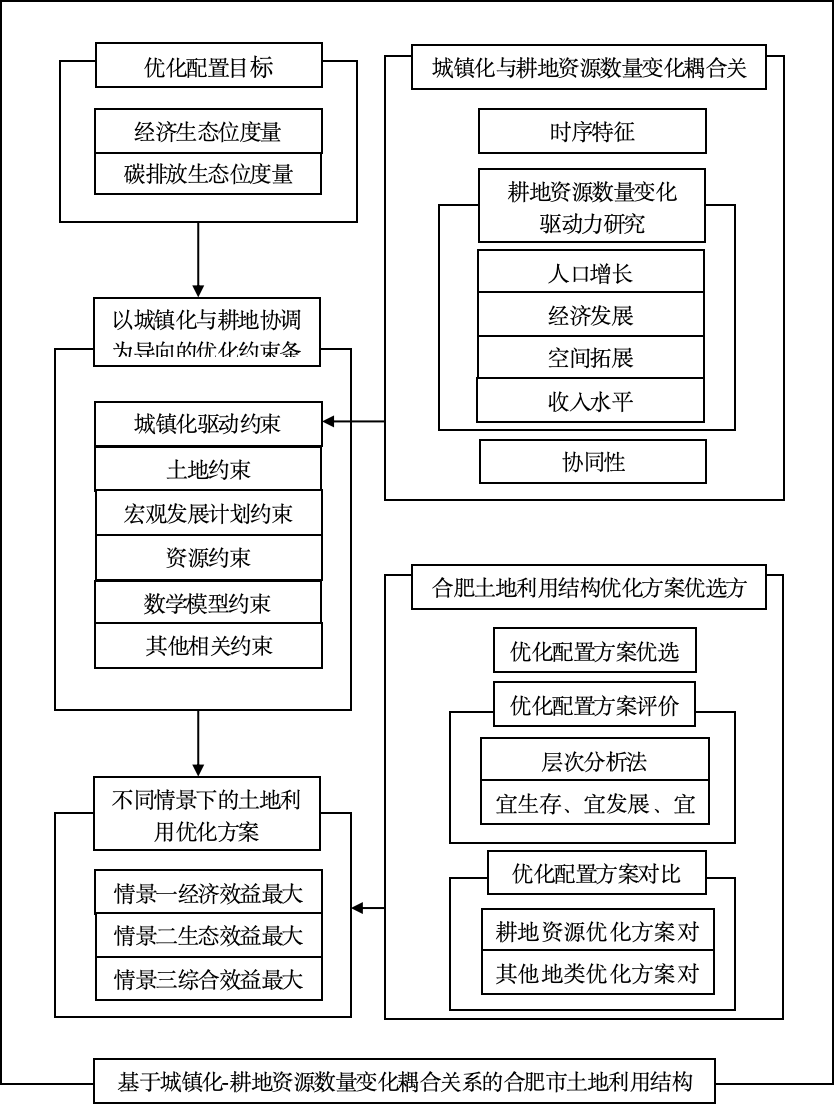
\includegraphics[width=1.0\textwidth]{../figure/图片2.png}
    \caption{技术路线图}
    \label{fig:tech-route}
    \centerline{Fig.\ 1.2 The technology roadmap}
\end{figure}

\clearpage\mbox{}\clearpage

\section{违章行为的心理原因问卷调查与因子分析研究}
\subsection{违章行为原因问卷编制与测试}
\subsubsection{违章行为主要原因归纳}

通过对国内外已有的有关个体违章行为研究的成果和事故案例及专家意见，将违章行为的主要原因归纳成如下十二个：

\dots\dots\dots\dots\dots\dots\dots\dots\dots\dots\dots\dots\dots\dots\dots\dots\dots\dots\dots\dots\dots\dots\dots\dots\dots\dots

上述计算方法所求出的主成分数量多时，可与原有指标相等。此时就反映了原有指标的全部信息，但没有减少指标，并非我们的目的。我们的目标是尽量用少数几个主成分反映指标的绝大多数的信息。如果 $Z_1, Z_2, Z_3, \dots, Z_p (p \le n)$ 的累计贡献率已达到 85\% 以上，这意味着前 $p$ 个主成分已能反映原有变量的绝大部分信息。

在主成分分析中将涉及到下列名词，先分别说明：
(1) 相关矩阵
即原指标 $x_1, x_2, x_3, \dots, x_n$ 首先标准化，然后求两两之间的相关系数组成的矩阵：
\begin{equation}
    \mathbf{R} = (r_{ij})_{m \times m}
\end{equation}
其中，相关矩阵为：
\begin{equation}
    \mathbf{R} = 
    \begin{bmatrix}
        r_{11} & r_{12} & r_{13} & \cdots & r_{1m} \\
        r_{21} & r_{22} & r_{23} & \cdots & r_{2m} \\
        r_{31} & r_{32} & r_{33} & \cdots & r_{3m} \\
        \cdots & \cdots & \cdots & \cdots & \cdots \\
        r_{m1} & r_{m2} & r_{m3} & \cdots & r_{mm} 
    \end{bmatrix}
\end{equation}

(2) 特征根
即根据上述矩阵得到的特征方程：
\begin{equation}
    | \mathbf{R} - \lambda \mathbf{I} | = 
    \begin{vmatrix}
        r_{11}-\lambda & r_{12} & \cdots & r_{1m} \\
        r_{21} & r_{22}-\lambda & \cdots & r_{2m} \\
        r_{31} & r_{32} & r_{33}-\lambda & \cdots \\
        \cdots & \cdots & \cdots & \cdots \\
        r_{m1} & r_{m2} & \cdots & r_{mm}-\lambda
    \end{vmatrix} = 0
\end{equation}

式中：\dots\dots

使上述行列式等于零，可得 $\lambda$ 的 $n$ 次方程，称为特征方程：
\begin{equation}
    \lambda^m - C_1 \lambda^{m-1} + C_2 \lambda^{m-2} + \dots + (-1)^{m-1} C_{m-1} \lambda + (-1)^m C_m = 0
\end{equation}

可解得 $m$ 个特征根，并使其按大小从大到小排序，得到：
\begin{equation}
    \lambda_1 \ge \lambda_2 \ge \lambda_3 \ge \dots \ge \lambda_m \ge 0
\end{equation}

(3) 特征根的贡献率
主成分 $Z_k$ 的贡献率为：
\begin{equation}
    \frac{\lambda_k}{\sum_{i=1}^m \lambda_i}
\end{equation}

前 $q$ 个主成分 $Y_1, Y_2, \dots, Y_q$ 的累计贡献率为：
\begin{equation}
    \frac{\sum_{i=1}^q \lambda_i}{\sum_{i=1}^m \lambda_i}
\end{equation}

\dots\dots\dots\dots\dots\dots\dots\dots

\section{结论与展望}

充分运用煤地球化学、煤岩学、煤田地质学、岩石学和矿物学等理论知识，通过大量的精密测试和系统分析，较为详细研究了煤中伴生元素的地质地球化学习性和成因机理，归纳了煤中伴生元素富集的地质模式。有如下认识：

(1) 通过对华北聚煤盆地一些典型矿区晚古生代煤中伴生元素的综合研究，并在充分收集前人研究工作的基础上，发现现局部地区外，华北聚煤盆地晚古生代煤中明显有害元素含量导因素。从现在掌握的资料来看，后期的岩浆热液和岩浆接触变质对煤的变质程度起了巨大作用，而对有害微量元素在煤中的富集作用仅在少数地区得到证实。

(2) 对全国晚古生代 226 个煤样中稀土元素的含量进行了统计，分析了煤中稀土元素的分布特征。

\dots\dots\dots\dots\dots\dots\dots\dots\dots\dots\dots\dots\dots\dots\dots\dots\dots\dots\dots\dots\dots\dots

(6) 研究发现，煤中稀土元素的含量主要受控于陆源碎屑的供给，山西组煤中稀土元这和煤层中稀土元素的赋存状态不同，表明不同的沉积环境以及相同的沉积环境对不同的物质中的稀土元素的分馏效应是不同的。

通过大量系统的研究工作，作者取得了一些有意义的认识。首次详细讨论了煤中铂族元素的含量和地质成因，在低温热液流体对煤中伴生元素的再分配作用等方面提出了新的见解和思路。希望最终能得到一个圆满的结论。

\clearpage
\mbox{}
\clearpage 
